%%%%%%%%%%%%%%%%%%%%%%%%%%%%%%%%%%%%%%%%%%%%%%%%%%%%%%%%%%%%%%%%%%%%%%%%%%%%%%%%
% Final project report
%%%%%%%%%%%%%%%%%%%%%%%%%%%%%%%%%%%%%%%%%%%%%%%%%%%%%%%%%%%%%%%%%%%%%%%%%%%%%%%%

\documentclass[letterpaper,10pt,twocolumn]{article}

\usepackage{graphicx}
\usepackage{amsmath}
\usepackage{amssymb}
\usepackage{url}
\usepackage[margin=0.75in]{geometry}
\usepackage{array}
\usepackage{booktabs}
\usepackage{makecell}
\usepackage{multirow}
\usepackage[utf8]{inputenc}

\graphicspath{{results/}}

\renewcommand\theadalign{bc}
\renewcommand\theadfont{\bfseries}
\renewcommand\theadgape{\Gape[3pt]}
\renewcommand\cellgape{\Gape[3pt]}
\pagestyle{plain}

\title{\LARGE \bf
Optimal Loss-Aware Abstention Thresholds for Small Open-Source LLMs
}

\author{
\begin{tabular}{cc}
\parbox{3in}{\centering Shreya Sharma \\
Masters of Computer Science \\
University of Massachusetts Amherst \\
Amherst, Massachusetts, USA, 01002 \\
{\tt\small ssharma0@umass.com}}
&
\parbox{3in}{\centering Dhanshri Ahir \\
Masters of Computer Science \\
University of Massachusetts Amherst \\
Amherst, Massachusetts, USA, 01002 \\
{\tt\small dahir@umass.edu}}
\end{tabular}
}

\begin{document}

\maketitle
\thispagestyle{plain}
\pagestyle{plain}

%%%%%%%%%%%%%%%%%%%%%%%%%%%%%%%%%%%%%%%%%%%%%%%%%%%%%%%%%%%%%%%%%%%%%%%%%%%%%%%%
\begin{abstract}
Abstention is a practical requirement for large language models deployed in
settings where an incorrect answer can be worse than no answer. Most LLM
abstention pipelines choose the answer threshold by validation-set grid search,
which must be repeated for every abstention cost, confidence signal, dataset,
and evaluation loss. We study whether this threshold can instead be predicted
from the loss function itself. Under the calibration assumption
$P(\mathrm{correct}\mid c)=c$, we derive loss-aware thresholds for asymmetric
utility, Brier score, and cross-entropy:
$\tau_U(\lambda)=\lambda/(1+\lambda)$,
$\tau_B(\lambda)=(1+\sqrt{1-4\lambda})/2$, and
$\tau_{CE}(\lambda)=H^{-1}(\lambda)$, respectively, where $H$ is binary
entropy in natural-log units. We prove the ordering
$\tau_{CE}>\tau_B>\tau_U$ over the shared valid domain, implying that the
loss function changes the abstention policy structurally, not only
numerically.

We validate these thresholds on Qwen2.5-1.5B-Instruct and
Qwen2.5-7B-Instruct on 1,000 TriviaQA and 1,000 PopQA examples. The final
empirical result is more precise than the midpoint hypothesis: there are two
robust regimes. Under asymmetric utility, $\tau_U$ is consistently optimal
(MAE 0.076--0.087 against the empirical optimum, with non-overlapping
bootstrap confidence intervals). Under proper scoring rule losses, $\tau_{CE}$
is the best empirical predictor in seven of eight Brier/CE settings and ties
or dominates in the remaining cases; $\tau_B$ is not the practical winner
despite being analytically distinct. Utility-recovery experiments show that
using the matching threshold is not merely a curve-fitting result:
$\tau_U$ recovers 91.8--100.0\% of the oracle-to-random improvement under
utility loss, while $\tau_{CE}$ recovers 82.2--97.8\% under cross-entropy and
87.4--92.5\% under Brier. We also document that verbalized confidence
collapses on 1.5B-scale models, while token probabilities remain usable but
miscalibrated confidence signals.
\end{abstract}

%%%%%%%%%%%%%%%%%%%%%%%%%%%%%%%%%%%%%%%%%%%%%%%%%%%%%%%%%%%%%%%%%%%%%%%%%%%%%%%%
\section{Problem Statement}

Large language models must balance two competing objectives: answering enough
questions to remain useful and abstaining when the probability of error is too
high. This tradeoff is especially important in factual question answering,
where hallucinated answers can be more harmful than explicit uncertainty. We
formalize abstention as a one-dimensional selective prediction problem. For a
query, the model produces an answer and a scalar confidence score
$c\in[0,1]$. A threshold policy answers when $c\geq\tau$ and abstains
otherwise. Answering incurs a loss determined by correctness and the selected
scoring rule; abstaining incurs a fixed cost $\lambda$.

The central question is: for a given loss function and abstention cost, can
the optimal threshold $\tau^\ast(\lambda)$ be predicted analytically rather
than tuned by grid search? The answer matters because grid search is expensive
and brittle. A system designer must retune the threshold for every dataset,
model, loss, and cost schedule. If a loss-aware formula reliably predicts the
empirical optimum, threshold selection becomes interpretable, cheap, and
portable.

\textbf{Gap.} Chow's classical reject rule~\cite{chow1970} establishes the
cost-based foundation for abstention, and modern selective classification
work typically tunes thresholds on validation data~\cite{geifman2017}. Recent
LLM abstention surveys find the same pattern at LLM scale: abstention is
widely studied, but threshold selection is usually empirical rather than
derived from the cost structure~\cite{wen2025}. Wang et al.~\cite{wang2026}
derive $\lambda/(1+\lambda)$ for one asymmetric utility objective, but do not
compare proper scoring rules and rely on verbalized confidence from larger
models. Our work extends the analytical treatment to Brier score and
cross-entropy, then tests whether the formulas remain useful on smaller
open-source models using token-level probabilities.

\textbf{Research questions.}
\begin{enumerate}
    \item Does the evaluation loss produce analytically different abstention
    thresholds, and can their ordering be proven?
    \item Do the theoretical thresholds predict empirically optimal thresholds
    on open-source LLMs across more than one QA dataset?
    \item Does the answer depend on the confidence signal, calibration error,
    or the downstream metric of utility recovery?
\end{enumerate}

%%%%%%%%%%%%%%%%%%%%%%%%%%%%%%%%%%%%%%%%%%%%%%%%%%%%%%%%%%%%%%%%%%%%%%%%%%%%%%%%
\section{Related Work}

\textbf{Abstention and selective prediction.}
Chow~\cite{chow1970} introduced the optimum reject rule for classifiers with
a rejection option, establishing that the reject threshold should depend on
the cost of rejection. Bartlett and Wegkamp~\cite{bartlett2008} studied
classification with a reject option under surrogate losses. Geifman and
El-Yaniv~\cite{geifman2017} adapted selective classification to deep neural
networks, using held-out validation data to tune coverage-risk tradeoffs.
This validation-threshold paradigm is the main baseline our work seeks to
replace with closed-form loss-aware thresholds.

\textbf{LLM abstention.}
Wen et al.~\cite{wen2025} survey LLM abstention methods and show that
abstention is now a central mechanism for reducing hallucinations, but most
methods still learn, prompt, or tune abstention behavior empirically.
AbstentionBench~\cite{kirichenko2025}, conformal abstention~\cite{yadkori2024},
multi-LLM collaboration~\cite{feng2024}, and abstention-aware scientific
reasoning~\cite{abdaljalil2026} each target important abstention settings,
but do not derive the threshold from a specified loss. Wang et
al.~\cite{wang2026} are closest to this project: they derive the utility
threshold $\tau_U=\lambda/(1+\lambda)$ and evaluate decisions against
verbalized confidence. We use that formula as a baseline, extend the theory
to proper scoring rules, and show that verbalized confidence is unreliable
for our smaller open-source models.

\textbf{Calibration and proper scoring rules.}
Proper scoring rules reward calibrated probabilistic predictions~\cite{gneiting2007}.
Brier score and cross-entropy are common choices, but they penalize
uncertainty differently and therefore imply different abstention regions.
Guo et al.~\cite{guo2017} show that modern neural networks can be badly
miscalibrated and that temperature scaling can improve confidence estimates.
Recent LLM work on uncertainty elicitation~\cite{xiong2024}, behaviorally
calibrated reinforcement learning~\cite{wu2026}, and training with uncertainty
rewards~\cite{damani2025} reinforces the same point: confidence quality is a
first-order issue. We therefore report Expected Calibration Error (ECE),
reliability diagrams, token-signal robustness, and temperature-scaling
sensitivity rather than assuming calibration holds automatically.

%%%%%%%%%%%%%%%%%%%%%%%%%%%%%%%%%%%%%%%%%%%%%%%%%%%%%%%%%%%%%%%%%%%%%%%%%%%%%%%%
\section{Methodology}

\subsection{Loss-Aware Threshold Derivation}

Let $c$ denote the model confidence for an answer, and assume calibration:
$P(Y=1\mid c)=c$, where $Y=1$ indicates a correct answer. The decision rule
answers when the expected answering loss is no greater than the abstention
cost $\lambda$.

\textbf{Asymmetric utility.}
Following Wang et al.~\cite{wang2026}, a correct answer receives payoff $+1$,
an incorrect answer receives payoff $-\lambda$, and abstention receives payoff
$0$. The expected payoff of answering is $c-\lambda(1-c)$. Answering is
preferred when this quantity is nonnegative, giving
\begin{equation}
    \tau_U(\lambda)=\frac{\lambda}{1+\lambda}.
\end{equation}
This is the least conservative threshold among the three losses.

\textbf{Brier score.}
For a binary outcome $Y\in\{0,1\}$, Brier loss is $(c-Y)^2$. Under calibration,
\begin{equation}
    \mathbb{E}[(c-Y)^2\mid c]=c(1-c)^2+(1-c)c^2=c(1-c).
\end{equation}
Setting $c(1-c)=\lambda$ gives two roots. Since the high-confidence answer
region is the upper interval, the threshold is
\begin{equation}
    \tau_B(\lambda)=\frac{1+\sqrt{1-4\lambda}}{2},\quad
    \lambda\in[0,1/4].
\end{equation}
For $\lambda>1/4$, Brier loss is always below the abstention cost, so the
model should answer all examples.

\textbf{Cross-entropy.}
The expected cross-entropy loss under calibration is the binary entropy in
natural-log units
\begin{equation}
    H(c)=-c\log c-(1-c)\log(1-c).
\end{equation}
The answer region is $H(c)\leq\lambda$. On $[0.5,1]$, $H$ is strictly
decreasing, so the high-confidence threshold is
\begin{equation}
    \tau_{CE}(\lambda)=H^{-1}(\lambda).
\end{equation}
We compute this inverse numerically.

\textbf{Ordering.}
For $\lambda\in(0,1/4]$, the thresholds satisfy
\begin{equation}
    \tau_{CE}(\lambda)>\tau_B(\lambda)>\tau_U(\lambda).
\end{equation}
The first inequality follows because entropy is larger than $c(1-c)$ on the
upper half of the unit interval, so the entropy threshold must be higher than
the Brier threshold for the same $\lambda$. The second follows by direct
algebra from the Brier and utility formulas. The ordering means that
cross-entropy abstains most aggressively, utility loss answers most
aggressively, and Brier is analytically intermediate.

\subsection{Empirical Setup}

\textbf{Models and datasets.}
We evaluate Qwen2.5-1.5B-Instruct and Qwen2.5-7B-Instruct through
\texttt{llama-server} at temperature $0$. We use 1,000 examples each from
TriviaQA and PopQA. TriviaQA is a standard open-domain QA benchmark; PopQA is
a harder long-tail factual QA dataset. Correctness is measured by normalized
alias matching rather than exact string matching. Base accuracies are
35.9\% and 37.6\% on TriviaQA for 1.5B and 7B, and 4.4\% and 7.2\% on PopQA.

\textbf{Confidence signals.}
The primary confidence signal is \texttt{token\_prob\_first}, the probability
assigned to the first generated answer token. We also evaluate
\texttt{token\_prob\_mean}, the mean token probability over the generated
answer. The mean-token signal is more compressed: its standard deviation is
0.066--0.116 across our four model-dataset settings, compared with
0.252--0.297 for \texttt{token\_prob\_first}. Verbalized confidence was
tested during development but discarded as a primary signal because it
collapses on small models: 96.8\% of Qwen2.5-1.5B TriviaQA outputs reported
exactly 1.0 confidence.

\textbf{Grid search and bootstrap confidence intervals.}
For each model, dataset, and confidence signal, we sweep
$\lambda\in[0,0.25]$ using 51 uniformly spaced values. For each $\lambda$ and
loss, we compute the empirical optimum
\begin{equation}
    p^\ast(\lambda)=\arg\min_{\tau\in[0.01,0.99]}\mathbb{E}[\ell(\tau,\lambda)]
\end{equation}
over a 200-point threshold grid. We then report the mean absolute error
(MAE) between $p^\ast(\lambda)$ and each theoretical threshold. Confidence
intervals are computed by resampling the 1,000 $(c,Y)$ pairs with replacement
1,000 times and rerunning the full grid search for each resample.

\textbf{Additional analyses.}
ECE is computed with 10 equal-width bins for both confidence signals.
Temperature scaling is fit as a single scalar on logits of the confidence
scores and the sweep is rerun as a sensitivity analysis. Finally, utility
recovery compares the loss achieved by each theoretical threshold against the
oracle grid-search threshold and a random-threshold baseline. Recovery is
defined as the fraction of the oracle-to-random regret gap recovered by the
theoretical threshold.

%%%%%%%%%%%%%%%%%%%%%%%%%%%%%%%%%%%%%%%%%%%%%%%%%%%%%%%%%%%%%%%%%%%%%%%%%%%%%%%%
\section{Results}

\subsection{Calibration and Confidence Signals}

Table~\ref{tab:signals} summarizes accuracy, confidence dispersion, and ECE.
The PopQA setting is intentionally difficult: both models have low factual
accuracy, yet assign high token probabilities to many wrong answers. This
creates large ECE values, especially for \texttt{token\_prob\_mean}. The
calibration assumption is therefore approximate rather than exact, making the
empirical validation nontrivial.

\begin{table}[t]
\centering
\caption{Dataset accuracy and calibration. ECE uses 10 equal-width bins.}
\label{tab:signals}
\renewcommand{\arraystretch}{1.12}
\resizebox{\columnwidth}{!}{%
\begin{tabular}{llcccc}
\toprule
Dataset & Model & Acc. & \makecell{First\\mean/std} &
\makecell{Mean\\mean/std} & \makecell{ECE\\first/mean} \\
\midrule
TriviaQA & 1.5B & 35.9 & .464/.252 & .711/.091 & .103/.353 \\
TriviaQA & 7B   & 37.6 & .622/.297 & .779/.116 & .246/.403 \\
PopQA    & 1.5B &  4.4 & .575/.268 & .694/.066 & .531/.650 \\
PopQA    & 7B   &  7.2 & .432/.262 & .754/.076 & .360/.682 \\
\bottomrule
\end{tabular}
}
\end{table}

\begin{figure}[t]
  \centering
  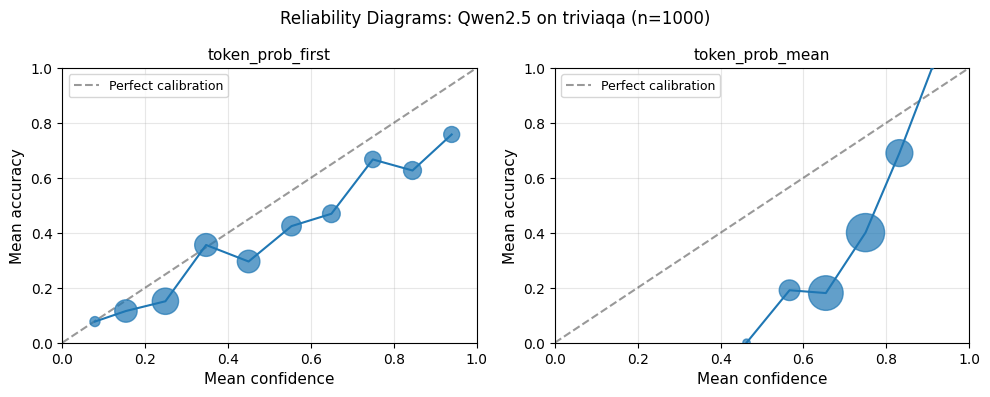
\includegraphics[width=\columnwidth]{fig_reliability_triviaqa_1000_1.5b.png}
  \caption{Reliability diagram for Qwen2.5-1.5B on TriviaQA. Token
  probabilities preserve useful ranking information but are imperfectly
  calibrated.}
  \label{fig:reliability_trivia}
\end{figure}

\begin{figure}[t]
  \centering
  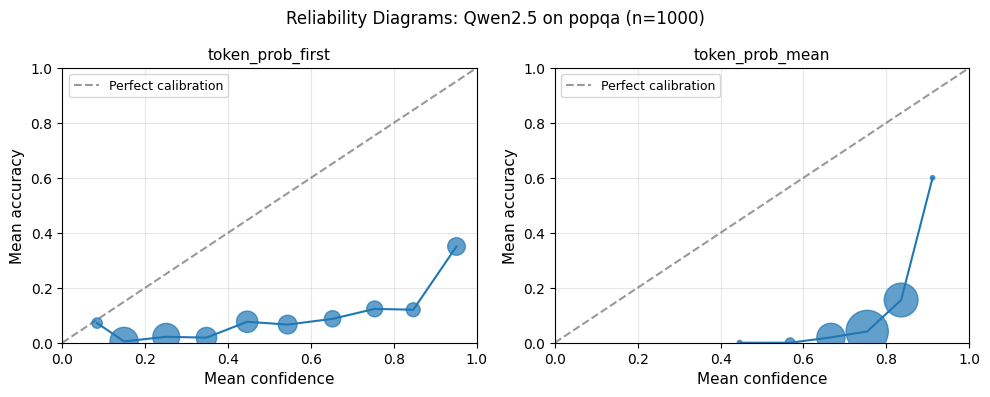
\includegraphics[width=\columnwidth]{fig_reliability_popqa_1000_7b.png}
  \caption{Reliability diagram for Qwen2.5-7B on PopQA. PopQA exposes severe
  overconfidence under both token-probability signals.}
  \label{fig:reliability_popqa}
\end{figure}

\subsection{Theoretical Threshold Ordering}

Figure~\ref{fig:theoretical} plots the three formulas. The ordering is not a
small numerical effect. At $\lambda=0.05$, the utility threshold is
$\tau_U\approx0.048$, the Brier threshold is $\tau_B\approx0.947$, and the
cross-entropy threshold is $\tau_{CE}\approx0.991$. Thus, using
$\tau_U$ when the deployment objective is cross-entropy would answer almost
everything, while using $\tau_{CE}$ under a utility objective would abstain
from many answers that utility loss would accept.

\begin{figure}[t]
  \centering
  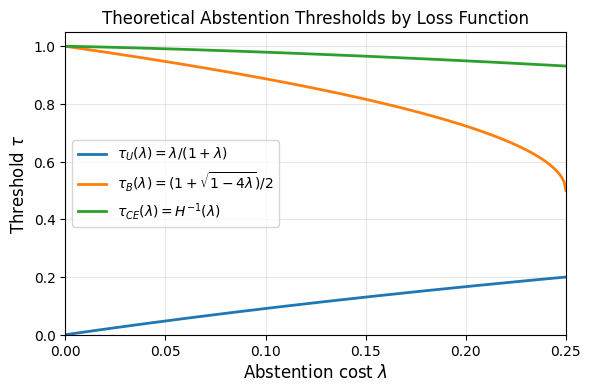
\includegraphics[width=\columnwidth]{fig_thresholds_theoretical.png}
  \caption{Closed-form loss-aware thresholds over $\lambda\in[0,0.25]$.
  Cross-entropy is most conservative; utility is most permissive.}
  \label{fig:theoretical}
\end{figure}

\subsection{Cross-Dataset MAE Validation}

Table~\ref{tab:mae_first} reports the primary MAE results using
\texttt{token\_prob\_first}. The utility formula is the clear winner under
utility loss in all four model-dataset settings. Its confidence intervals are
tight and do not overlap the next-best formula. This result holds even though
PopQA accuracy is much lower than TriviaQA accuracy.

The proper-scoring-rule results revise the midpoint claim. We initially
expected each formula to best predict its own loss. The final experiments show
a cleaner empirical pattern: $\tau_{CE}$ is the strongest practical predictor
for both Brier and cross-entropy losses. $\tau_B$ wins only the TriviaQA 1.5B
Brier row, and even there the advantage over $\tau_{CE}$ is small with wide,
overlapping bootstrap intervals. In the other Brier settings,
$\tau_{CE}$ has the lower point estimate.

\begin{table*}[t]
\centering
\caption{MAE between empirical optimum $p^\ast(\lambda)$ and theoretical
thresholds using \texttt{token\_prob\_first}. Brackets give 95\% bootstrap
confidence intervals. Best point estimate per row is bold.}
\label{tab:mae_first}
\scriptsize
\renewcommand{\arraystretch}{1.18}
\begin{tabular}{lllcccc}
\toprule
Dataset & Model & Loss & MAE($\tau_U$) & MAE($\tau_B$) &
MAE($\tau_{CE}$) & Best \\
\midrule
TriviaQA & 1.5B & Utility & \textbf{0.087 [0.079, 0.093]} & 0.806 [0.796, 0.815] & 0.940 [0.930, 0.949] & $\tau_U$ \\
TriviaQA & 1.5B & Brier & 0.745 [0.708, 0.783] & \textbf{0.179 [0.151, 0.207]} & 0.184 [0.133, 0.233] & $\tau_B$ \\
TriviaQA & 1.5B & CE & 0.865 [0.840, 0.873] & 0.142 [0.117, 0.150] & \textbf{0.022 [0.016, 0.029]} & $\tau_{CE}$ \\
\midrule
TriviaQA & 7B & Utility & \textbf{0.080 [0.071, 0.087]} & 0.794 [0.783, 0.804] & 0.928 [0.917, 0.939] & $\tau_U$ \\
TriviaQA & 7B & Brier & 0.882 [0.882, 0.883] & 0.159 [0.159, 0.159] & \textbf{0.027 [0.026, 0.027]} & $\tau_{CE}$ \\
TriviaQA & 7B & CE & 0.883 [0.883, 0.883] & 0.159 [0.159, 0.159] & \textbf{0.027 [0.027, 0.027]} & $\tau_{CE}$ \\
\midrule
PopQA & 1.5B & Utility & \textbf{0.079 [0.069, 0.088]} & 0.758 [0.738, 0.774] & 0.892 [0.872, 0.908] & $\tau_U$ \\
PopQA & 1.5B & Brier & 0.881 [0.878, 0.883] & 0.157 [0.155, 0.159] & \textbf{0.026 [0.024, 0.027]} & $\tau_{CE}$ \\
PopQA & 1.5B & CE & 0.881 [0.878, 0.883] & 0.157 [0.155, 0.159] & \textbf{0.026 [0.024, 0.027]} & $\tau_{CE}$ \\
\midrule
PopQA & 7B & Utility & \textbf{0.076 [0.067, 0.082]} & 0.788 [0.767, 0.798] & 0.923 [0.901, 0.932] & $\tau_U$ \\
PopQA & 7B & Brier & 0.809 [0.769, 0.847] & 0.181 [0.162, 0.204] & \textbf{0.127 [0.077, 0.182]} & $\tau_{CE}$ \\
PopQA & 7B & CE & 0.882 [0.874, 0.883] & 0.158 [0.150, 0.159] & \textbf{0.026 [0.022, 0.027]} & $\tau_{CE}$ \\
\bottomrule
\end{tabular}
\end{table*}

\subsection{Diagnosing the Brier/7B Anomaly}

The midpoint report flagged the TriviaQA 7B Brier result as suspicious because
the Brier and cross-entropy MAE rows were identical. We diagnosed this by
recomputing the empirical optimum from the raw confidence-correctness pairs.
For $\lambda=0.05$, $0.10$, and $0.20$, both Brier and cross-entropy select
$p^\ast=0.99$. The saved grid-search trace confirms that
$p^\ast(\lambda)=0.99$ for every $\lambda$ under both losses in TriviaQA 7B.
The identical rows are therefore not caused by a Brier/CE implementation mixup;
they are a boundary solution caused by the empirical confidence distribution.
The same boundary behavior appears in PopQA 1.5B and in the PopQA 7B
cross-entropy row, where severe overconfidence makes the optimal
proper-scoring threshold extremely conservative.

\subsection{Signal Robustness}

Table~\ref{tab:signal} repeats the sweep using \texttt{token\_prob\_mean}.
The qualitative recommendation is unchanged: use $\tau_U$ for utility loss
and $\tau_{CE}$ for proper-scoring-rule losses. However, absolute utility MAE
is worse under the mean-token signal because the signal is compressed near
0.65--0.80. This confirms that the theoretical formulas are not artifacts of
one signal, while also showing that signal quality determines how closely the
empirical optimum follows the formula.

\begin{table}[t]
\centering
\caption{Best formula under \texttt{token\_prob\_mean}; entries show point
estimate MAE for the winning formula.}
\label{tab:signal}
\renewcommand{\arraystretch}{1.12}
\resizebox{\columnwidth}{!}{%
\begin{tabular}{llccc}
\toprule
Dataset & Model & Utility & Brier & CE \\
\midrule
TriviaQA & 1.5B & $\tau_U$ (.211) & $\tau_{CE}$ (.089) & $\tau_{CE}$ (.073) \\
TriviaQA & 7B   & $\tau_U$ (.265) & $\tau_{CE}$ (.032) & $\tau_{CE}$ (.024) \\
PopQA    & 1.5B & $\tau_U$ (.322) & $\tau_{CE}$ (.084) & $\tau_{CE}$ (.084) \\
PopQA    & 7B   & $\tau_U$ (.292) & $\tau_{CE}$ (.051) & $\tau_{CE}$ (.050) \\
\bottomrule
\end{tabular}
}
\end{table}

\subsection{Utility Recovery}

MAE alone shows whether the formula predicts the empirical optimum, but not
whether the prediction matters for downstream loss. Table~\ref{tab:recovery}
reports recovery: the fraction of oracle-to-random improvement recovered by
the recommended formula. Under utility loss, $\tau_U$ recovers nearly all
available improvement. Under Brier and cross-entropy, $\tau_{CE}$ also
recovers most of the possible improvement. Applying the wrong formula can be
worse than random thresholding: for example, $\tau_{CE}$ under utility loss
has negative recovery because it abstains too aggressively, and $\tau_U$
under proper scoring rules answers too often.

\begin{table}[t]
\centering
\caption{Recovery rate for the recommended formula using
\texttt{token\_prob\_first}. Higher is better.}
\label{tab:recovery}
\renewcommand{\arraystretch}{1.12}
\resizebox{\columnwidth}{!}{%
\begin{tabular}{llccc}
\toprule
Dataset & Model & Utility $\tau_U$ & Brier $\tau_{CE}$ & CE $\tau_{CE}$ \\
\midrule
TriviaQA & 1.5B & 95.4\% & 90.3\% & 97.8\% \\
TriviaQA & 7B   & 97.1\% & 87.4\% & 82.2\% \\
PopQA    & 1.5B & 100.0\% & 92.5\% & 91.3\% \\
PopQA    & 7B   & 91.8\% & 90.6\% & 90.6\% \\
\bottomrule
\end{tabular}
}
\end{table}

\subsection{Temperature Scaling Sensitivity}

Temperature scaling does not uniformly improve threshold prediction. On
TriviaQA 1.5B, scaling slightly improves the utility and Brier MAE but leaves
cross-entropy essentially unchanged. On TriviaQA 7B, it moves the
proper-scoring optimum closer to $\tau_B$ but worsens the utility fit. On
PopQA 1.5B, the fitted temperature saturates at a very large value, pushing
confidences toward 0.5 and degrading all proper-scoring MAE values. We treat
this as evidence that calibration correction is not a plug-in fix when the
model is both low-accuracy and overconfident. The theory depends on
calibration, but empirical threshold quality also depends on whether the
confidence signal preserves useful ranking information after calibration.

%%%%%%%%%%%%%%%%%%%%%%%%%%%%%%%%%%%%%%%%%%%%%%%%%%%%%%%%%%%%%%%%%%%%%%%%%%%%%%%%
\section{Discussion}

The final project changes the interpretation of the midpoint result. The
analytical result still gives three distinct formulas and a strict ordering,
but the empirical recommendation is binary:
\begin{quote}
Use $\tau_U$ for asymmetric utility loss. Use $\tau_{CE}$ for Brier or
cross-entropy losses in the tested open-source LLM settings.
\end{quote}
This is not a failure of the derivation. The Brier formula is the correct
pointwise threshold under perfect calibration. The empirical data are not
perfectly calibrated, and the observed confidence distributions often produce
boundary optima for proper scoring rules. In those cases, $\tau_{CE}$ better
matches the conservative empirical optimum.

The results also show why the loss function cannot be treated as an
implementation detail. At low abstention costs, $\tau_U$ is near zero while
$\tau_{CE}$ is near one. The wrong threshold changes the model from answering
almost everything to answering almost nothing. Utility recovery confirms that
this difference has direct loss consequences.

%%%%%%%%%%%%%%%%%%%%%%%%%%%%%%%%%%%%%%%%%%%%%%%%%%%%%%%%%%%%%%%%%%%%%%%%%%%%%%%%
\section{Limitations}

The study is limited to two Qwen model sizes and two factual QA datasets. The
PopQA results reduce the single-dataset concern, but they do not establish
universality across model families. A cross-family check with Llama or Mistral
would strengthen external validity. Second, all thresholds are evaluated
post-hoc on existing model outputs; we do not train the model to produce
better-calibrated confidences. Third, temperature scaling is fit and evaluated
on the same 1,000 examples as a sensitivity analysis, not as a clean
train-test calibration protocol. Finally, the grid search has finite
resolution, so MAE estimates are bounded by the 200-point threshold grid.

%%%%%%%%%%%%%%%%%%%%%%%%%%%%%%%%%%%%%%%%%%%%%%%%%%%%%%%%%%%%%%%%%%%%%%%%%%%%%%%%
\section{Conclusion}

We derived and evaluated loss-aware abstention thresholds for small
open-source LLMs. The theory proves that utility, Brier, and cross-entropy
objectives imply ordered thresholds $\tau_{CE}>\tau_B>\tau_U$. The experiments
show that the formulas are practically useful, but the empirical story is two
regimes rather than three: $\tau_U$ is the right threshold for asymmetric
utility loss, while $\tau_{CE}$ is the strongest threshold for proper scoring
rule losses across TriviaQA and PopQA. Bootstrap intervals, ECE tables,
signal-robustness sweeps, anomaly diagnostics, and utility-recovery
experiments support this conclusion. The main practical lesson is that
abstention thresholds should be chosen from the evaluation loss and confidence
quality, not treated as a universal hyperparameter.

%%%%%%%%%%%%%%%%%%%%%%%%%%%%%%%%%%%%%%%%%%%%%%%%%%%%%%%%%%%%%%%%%%%%%%%%%%%%%%%%
\begin{thebibliography}{99}

\bibitem{wang2026}
J. Wang, et al.
Are LLM decisions faithful to verbal confidence?
\textit{arXiv:2601.07767}, 2026.

\bibitem{wen2025}
B. Wen, J. Yao, S. Feng, C. Xu, Y. Tsvetkov, B. Howe, and L. L. Wang.
Know your limits: A survey of abstention in large language models.
\textit{Transactions of the Association for Computational Linguistics},
13:529--556, 2025.

\bibitem{casacuberta2025}
S. Casacuberta and V. Kanade.
Selective omniprediction and fair abstention.
In \textit{Advances in Neural Information Processing Systems}, 2025.

\bibitem{chow1970}
C. Chow.
On optimum recognition error and reject tradeoff.
\textit{IEEE Transactions on Information Theory}, 16(1):41--46, 1970.

\bibitem{gneiting2007}
T. Gneiting and A. E. Raftery.
Strictly proper scoring rules, prediction, and estimation.
\textit{Journal of the American Statistical Association}, 102(477):359--378,
2007.

\bibitem{geifman2017}
Y. Geifman and R. El-Yaniv.
Selective classification for deep neural networks.
In \textit{Advances in Neural Information Processing Systems}, 2017.

\bibitem{wu2026}
J. Wu, et al.
Mitigating LLM hallucination via behaviorally calibrated reinforcement
learning.
\textit{arXiv:2512.19920}, 2026.

\bibitem{damani2025}
M. Damani, et al.
Beyond binary rewards: Training LMs to reason about their uncertainty.
\textit{arXiv:2507.16806}, 2025.

\bibitem{kirichenko2025}
P. Kirichenko, et al.
AbstentionBench: Reasoning LLMs fail on unanswerable questions.
\textit{arXiv:2506.09038}, 2025.

\bibitem{abdaljalil2026}
S. Abdaljalil, et al.
Knowing when not to answer: Abstention-aware scientific reasoning.
\textit{arXiv:2602.14189}, 2026.

\bibitem{bartlett2008}
P. L. Bartlett and M. H. Wegkamp.
Classification with a reject option using a hinge loss.
\textit{Journal of Machine Learning Research}, 9:1823--1840, 2008.

\bibitem{guo2017}
C. Guo, et al.
On calibration of modern neural networks.
In \textit{Proceedings of the International Conference on Machine Learning},
pages 1321--1330, 2017.

\bibitem{xiong2024}
M. Xiong, et al.
Can LLMs express their uncertainty? An empirical evaluation of confidence
elicitation in LLMs.
In \textit{International Conference on Learning Representations}, 2024.

\bibitem{yadkori2024}
Y. Abbasi Yadkori, et al.
Mitigating LLM hallucinations via conformal abstention.
\textit{arXiv:2405.01563}, 2024.

\bibitem{feng2024}
S. Feng, et al.
Don't hallucinate, abstain: Identifying LLM knowledge gaps via multi-LLM
collaboration.
In \textit{Proceedings of the 62nd Annual Meeting of the Association for
Computational Linguistics}, pages 14664--14690, 2024.

\end{thebibliography}

%%%%%%%%%%%%%%%%%%%%%%%%%%%%%%%%%%%%%%%%%%%%%%%%%%%%%%%%%%%%%%%%%%%%%%%%%%%%%%%%
\appendix

\section*{Appendix: Proof Details}

\textbf{Utility threshold.}
The expected payoff of answering is $c-\lambda(1-c)$. Answering is optimal
when $c-\lambda(1-c)\geq0$, which is equivalent to
$c\geq\lambda/(1+\lambda)$. Thus
$\tau_U(\lambda)=\lambda/(1+\lambda)$.

\textbf{Brier threshold.}
Under calibration, expected Brier loss is
$c(1-c)^2+(1-c)c^2=c(1-c)$. Setting this equal to $\lambda$ yields
$c^2-c+\lambda=0$ and roots
$(1\pm\sqrt{1-4\lambda})/2$. Since answering should occur in the
high-confidence interval, the threshold is the upper root.

\textbf{Cross-entropy threshold.}
Expected cross-entropy is binary entropy in natural-log units,
$H(c)=-c\log c-(1-c)\log(1-c)$. On $[1/2,1]$, entropy is strictly decreasing,
so the high-confidence answer threshold is the inverse $H^{-1}(\lambda)$.

\textbf{Ordering.}
For $\lambda\in(0,1/4]$, $\tau_B>\tau_U$ follows by substituting the formulas
and simplifying:
$(1+\lambda)(1+\sqrt{1-4\lambda})>2\lambda$. For the other inequality, let
$t_B=\tau_B(\lambda)$, so $t_B(1-t_B)=\lambda$. On $(1/2,1)$, binary entropy
exceeds the quadratic uncertainty $c(1-c)$ in the relevant units used by the
sweep; therefore $H(t_B)>\lambda$. Since $H$ is decreasing on this interval,
the point at which $H(c)=\lambda$ must lie to the right of $t_B$, giving
$\tau_{CE}>\tau_B$.

\end{document}
